% ************************************************************************
%
% Introduction
%
% ************************************************************************
\chpos{22mm}{10mm}
\chapter[Introduction]{Introduction}
\markboth{\thechapter\ \ Introduction}{\thechapter\ \ Introduction}
\label{ch1:introduction}

\mysquote{0.8\textwidth}
{Perfecting oneself is as much unlearning as it is learning.}
{Edsger Dijkstra (\oldstylenums{1930} - \oldstylenums{2002})}


% ************************************************************************
\section{Studying Neuron Cell} 
Some text \cite{abramoff2004image}. And \cite{ascolitrees}.


\section{Thesis Outline}
In this thesis... 
%\begin{figure}[!t]
%  \begin{center}
%  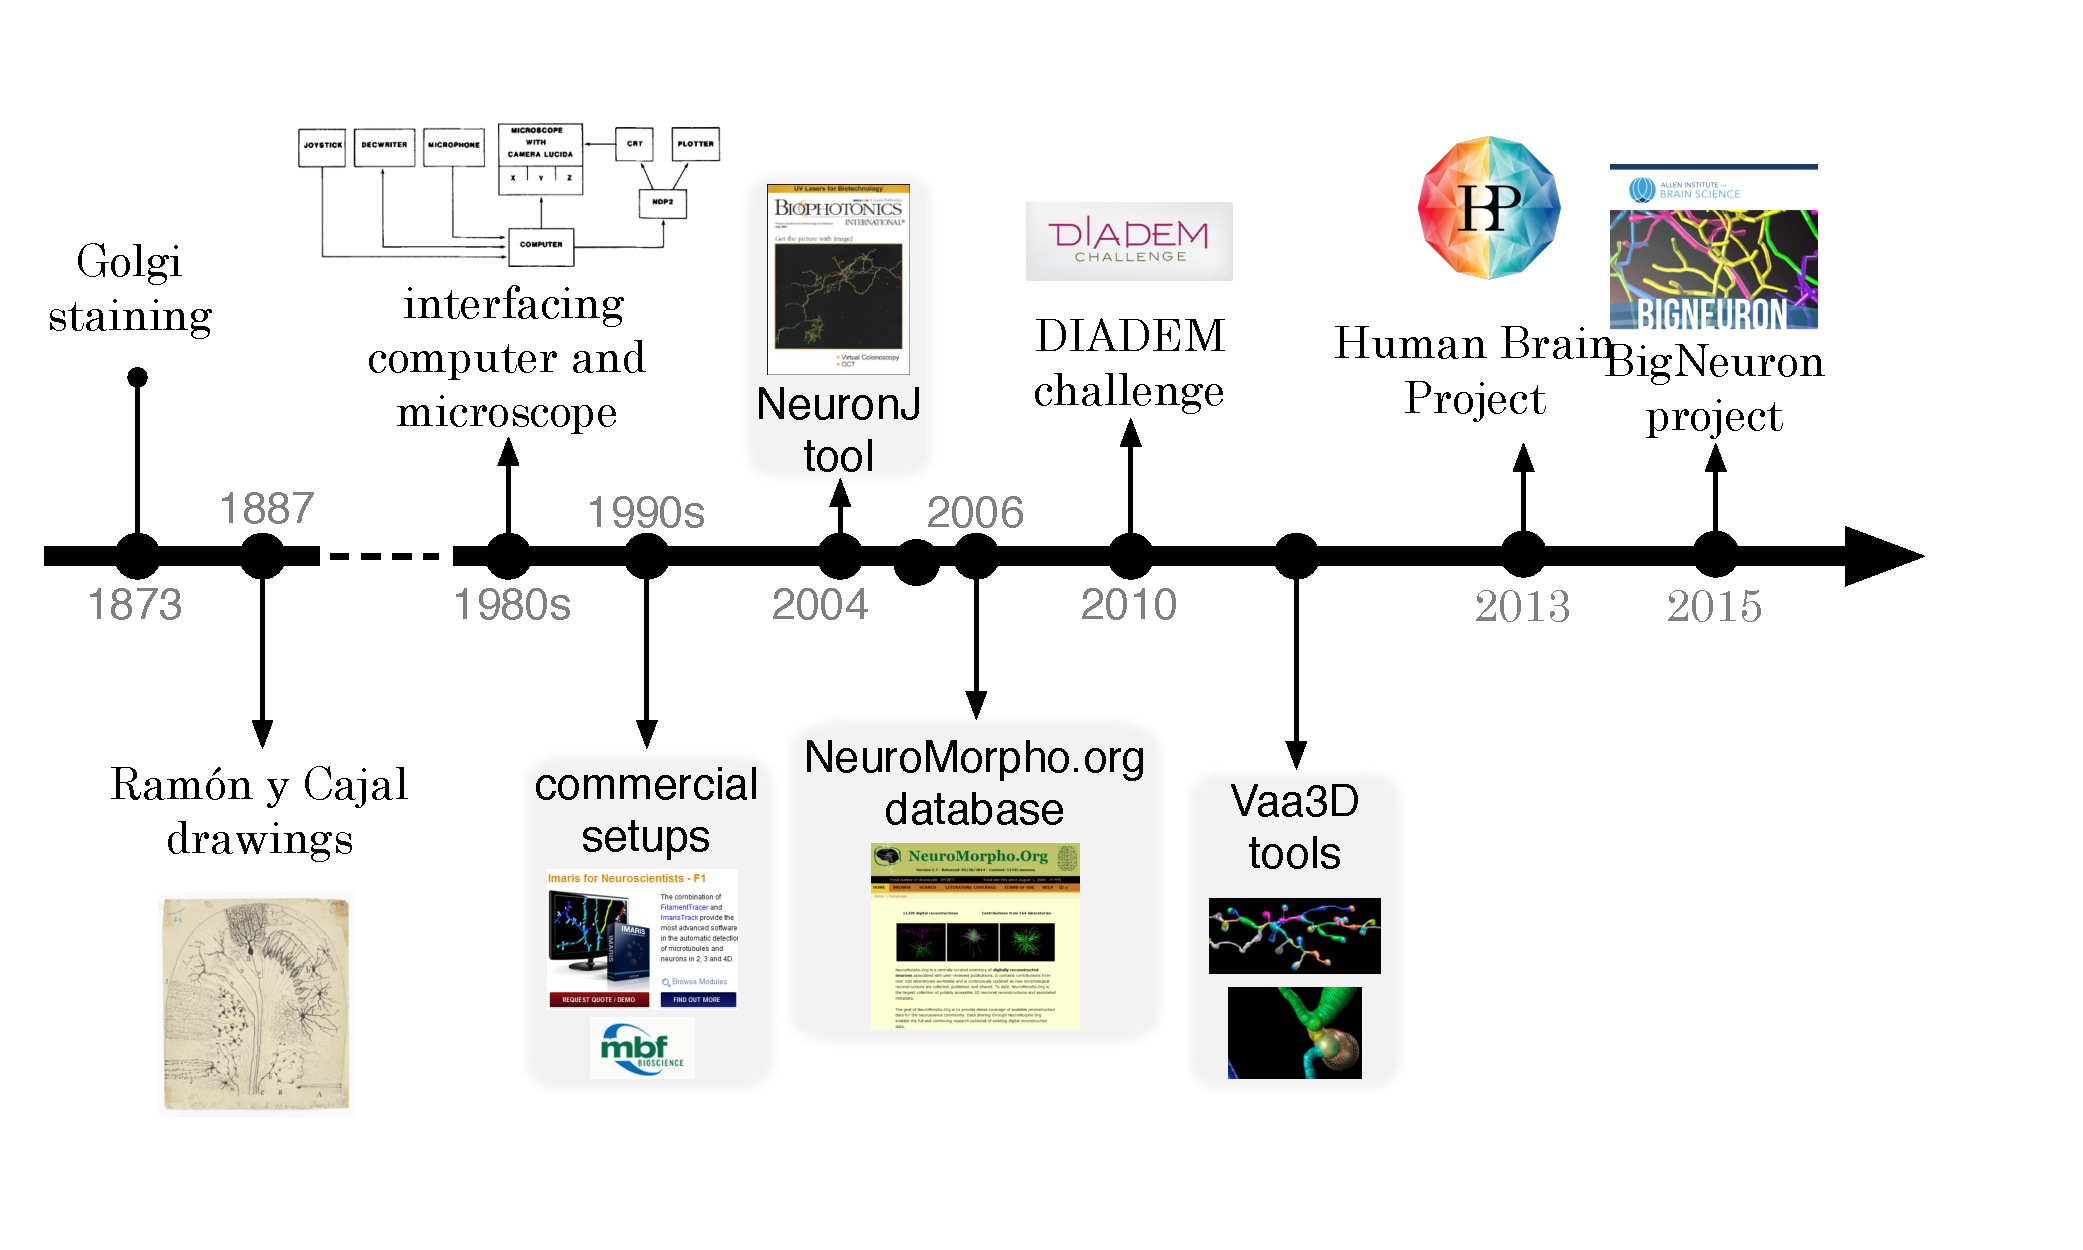
\includegraphics[width=\textwidth]{ch1_fig1}
%  \end{center}
%\vspace{-3ex}
%  \caption{Examples of images acquired for different biological
%    studies based on GFP labeling and fluorescence
%    microscopy. The images are single frames from 2D time-lapse
%    studies of activity of microtubule plus-ends (top left), microtubule
%    plus-ends in neurons (top right), Rab5 (bottom left) and
%    peroxisomes (bottom right).
%}
%\vspace{-1ex}
%\label{ch1__fig1}
%\end{figure}
